\section{Innledning}

Helsedirektoratet.no er en sentral informasjons- og kunnskapsplattform for helse- og omsorgssektoren i Norge, og brukes av både fagpersoner, offentlige aktører og privatpersoner. Nettstedet publiserer et stort volum innhold med ulike dokumenttyper og informasjonsbehov, noe som stiller høye krav til søk og navigasjon. Denne oppgaven undersøker hvordan gjenfinnbarheten kan forbedres gjennom en kombinasjon av Kunsti intelligens (KI) støttet søk og en mer støttende navigasjonsopplevelse.

\begin{figure}[H]
    \centering
    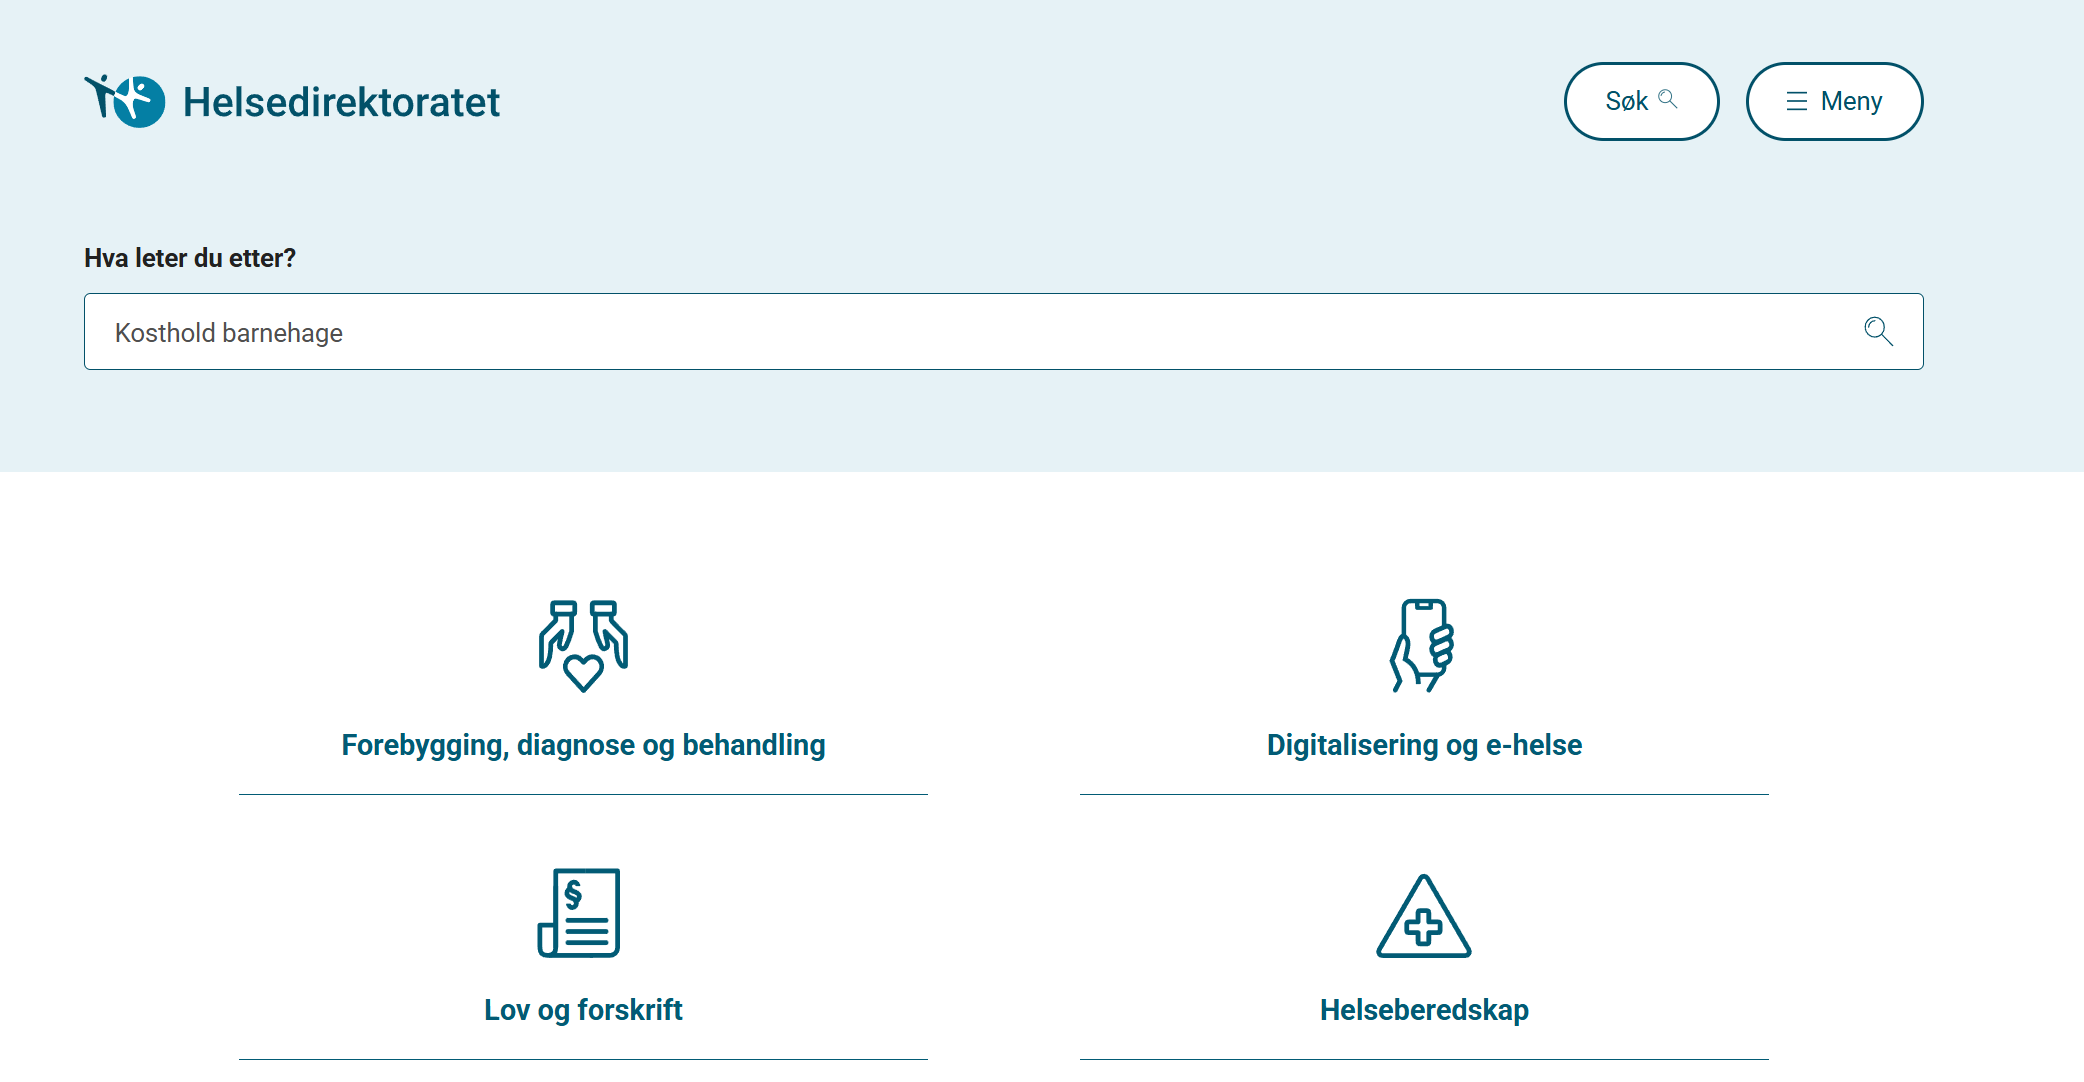
\includegraphics[width=\textwidth]{Images/helsedirektoratet.no/helsedirektoratet-forside.png}
    \caption{Forsiden på helsedirektoratet.no som viser to av syv temaside kategorier.}
    \label{fig:Helsedir-forside}
\end{figure}

Figur \ref{fig:Helsedir-forside} viser hva man møter når man åpner helsedirektoratet.no. Hovedoppsettet her er søkefunksjonaliteten og de forskjellige kategoriseringene av informasjon man kan navigere etter.  


\subsection{Helsedirektoratet.no}
\label{sec:helsedir}

Helsedirektoratet.no samler og formidler et bredt spekter av innhold, blant annet retningslinjer, anbefalinger, faglige råd og informasjon rettet mot befolkningen. Nettstedet betjener derfor mange ulike målgrupper med forskjellige behov og forutsetninger. Som vist i figur \ref{fig:helsedir-målgrupper} omfatter dette blant annet helsepersonell, offentlig forvaltning, forskere og privatpersoner.

Et sentralt problem er at informasjon kan være vanskelig å finne selv når den finnes på nettstedet. Dette kan skyldes flere forhold, som varierende terminologi mellom bruker og innhold, store dokumentmengder, komplekse relasjoner mellom hovedinnhold og underinnhold, samt utydelige navigasjonsvalg. Når brukere ikke finner relevant informasjon effektivt, øker tidsbruk og frustrasjon, og det kan skape barrierer for god informasjonsinnhenting og svekke opplevelsen av offentlige digitale tjenester.

\begin{figure}[H]
    \centering
    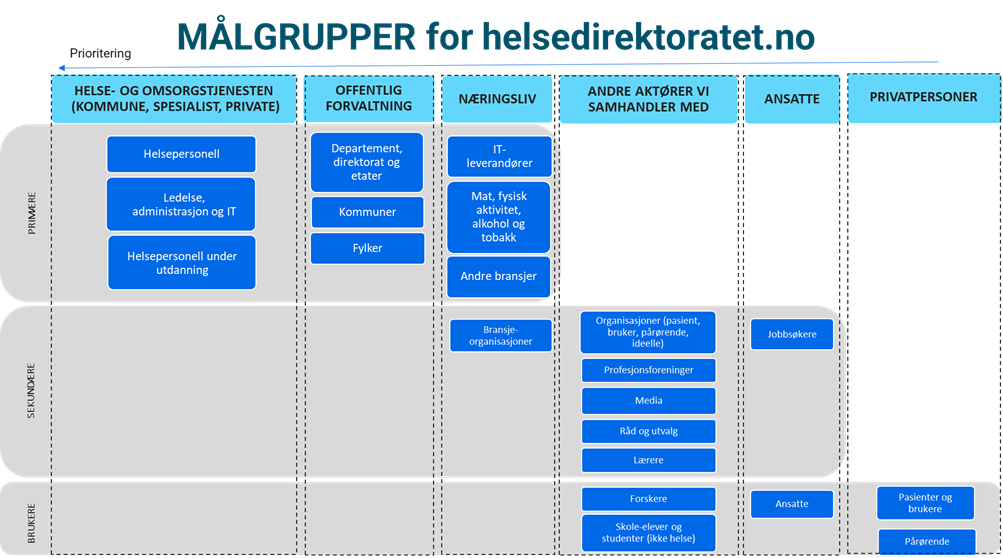
\includegraphics[width=\textwidth]{Images/MålgrupperHelseDir.png}
    \caption{Oversikt over målgruppene til helsedirektoratet.no.}
    \label{fig:helsedir-målgrupper}
\end{figure}

For en så heterogen målgruppe innebærer dette at én og samme søke- og navigasjonsløsning må håndtere både ulike fagbegreper, ulike informasjonsbehov og ulike forventninger til presisjon og forklarbarhet. Dette gjør helsedirektoratet.no til et egnet case for å undersøke hvordan AI-støttet informasjonsgjenfinning og mer kontekstuell navigasjon kan redusere friksjon i informasjonsinnhenting. I resten av innledningen presenteres oppdraget fra Helsedirektoratet, prosjektets mål og leveranser, samt rammer og avgrensninger for arbeidet.




\subsection{Oppdrag, mål og avgrensning}
\label{sec:oppdrag}

Bacheloroppgaven tar utgangspunkt i en oppgavebeskrivelse fra Helsedirektoratet. Formålet er å undersøke hvordan søk og navigasjon på helsedirektoratet.no kan forbedres ved hjelp av kunstig intelligens, og å demonstrere forbedringspotensialet gjennom utvikling og evaluering av en prototype.

Prosjektet adresserer to komplementære forbedringsområder: \textbf{søk}, som undersøkes gjennom KI-baserte mekanismer i backend (f.eks.\ semantisk informasjonsgjenfinning og støtte for varierende terminologi), og \textbf{navigasjon}, som undersøkes gjennom en GUI som tydeliggjør struktur, relasjoner og veivalg i innholdet. Arbeidet forankres i brukerinnsikt fra kartlegging av dagens løsning og evalueres gjennom en sammenligning mellom eksisterende løsning og prototype.


\subsection{Mål og leveranser}

Det overordnede målet med prosjektet er å undersøke hvordan kunstig intelligens kan bidra til forbedret søk og navigasjon på helsedirektoratet.no, og å demonstrere dette gjennom utvikling og evaluering av et konkret konsept eller en prototype.

\subsubsection{Hovedmål og delmål}
\label{sec:mal}

\textbf{Hovedmål:} Å undersøke hvordan kunstig intelligens kan bidra til forbedret søk og navigasjon på helsedirektoratet.no, og å demonstrere dette gjennom utvikling og evaluering av et konkret konsept eller en prototype.

\textbf{Delmål:}
\begin{itemize}
    \item Kartlegge og analysere eksisterende søkefunksjonalitet og navigasjonsstruktur på helsedirektoratet.no.
    \item Identifisere sentrale utfordringer knyttet til informasjonsgjenfinning for ulike brukergrupper gjennom brukerundersøkelser.
    \item Vurdere relevante KI-baserte tilnærminger, herunder semantisk søk og (der det er hensiktsmessig) automatisk kategorisering/tagging av innhold.
    \item Utforme en prototype eller et konsept som adresserer identifiserte utfordringer innen søk og navigasjon.
    \item Evaluere prototypen opp mot eksisterende løsning gjennom representative oppgaver og brukerinnsikt.
\end{itemize}



\subsubsection{Leveranser (resultatmål)}
\label{sec:leveranser}

Prosjektets leveranser består av:
\begin{itemize}
    \item en skriftlig bachelorrapport som dokumenterer metodikk, designvalg, evaluering og etiske vurderinger,
    \item en prototype/konseptuell løsning med tilhørende dokumentasjon,
    \item en analyse av dagens søk og navigasjon, inkludert identifiserte styrker og svakheter,
    \item en evaluering av foreslått løsning basert på relevans og brukervennlighet, støttet av brukerundersøkelser og/eller representative scenarier.
\end{itemize}

\subsubsection{Forventet effekt (effektmål)}
\label{sec:effektmal}

Prosjektet har som mål å bidra til følgende effekter:
\begin{itemize}
    \item forbedret opplevd relevans i søkeresultater og/eller høyere treffsikkerhet i representative oppgaver,
    \item redusert tid og/eller færre interaksjoner for å finne spesifikk informasjon i brukertester,
    \item økt opplevd brukervennlighet og brukertilfredshet målt gjennom spørreskjema etter testing,
    \item økt transparens og konsistens i organiseringen av innhold, støttet av tydeligere kontekst og (der det er relevant) strukturert metadata/tagging.
\end{itemize}

\subsubsection{Rammer og avgrensninger}
\label{sec:rammer}

Prosjektet gjennomføres innenfor rammene av en bacheloroppgave (22,5 studiepoeng) og er avgrenset til konseptuell utforming, prototyping og evaluering fremfor fullskala utvikling og produksjonssetting. Løsningen skal derfor betraktes som et \textit{proof of concept}.

Prosjektgruppen har ikke hatt tilgang til intern infrastruktur, kildekode eller produksjonsmiljøer tilknyttet helsedirektoratet.no. Prototypen baserer seg derfor på offentlig tilgjengelig informasjon og åpne API-er, og implementeres som en selvstendig løsning utviklet fra bunnen av.

\begin{figure}[H]
    \centering
    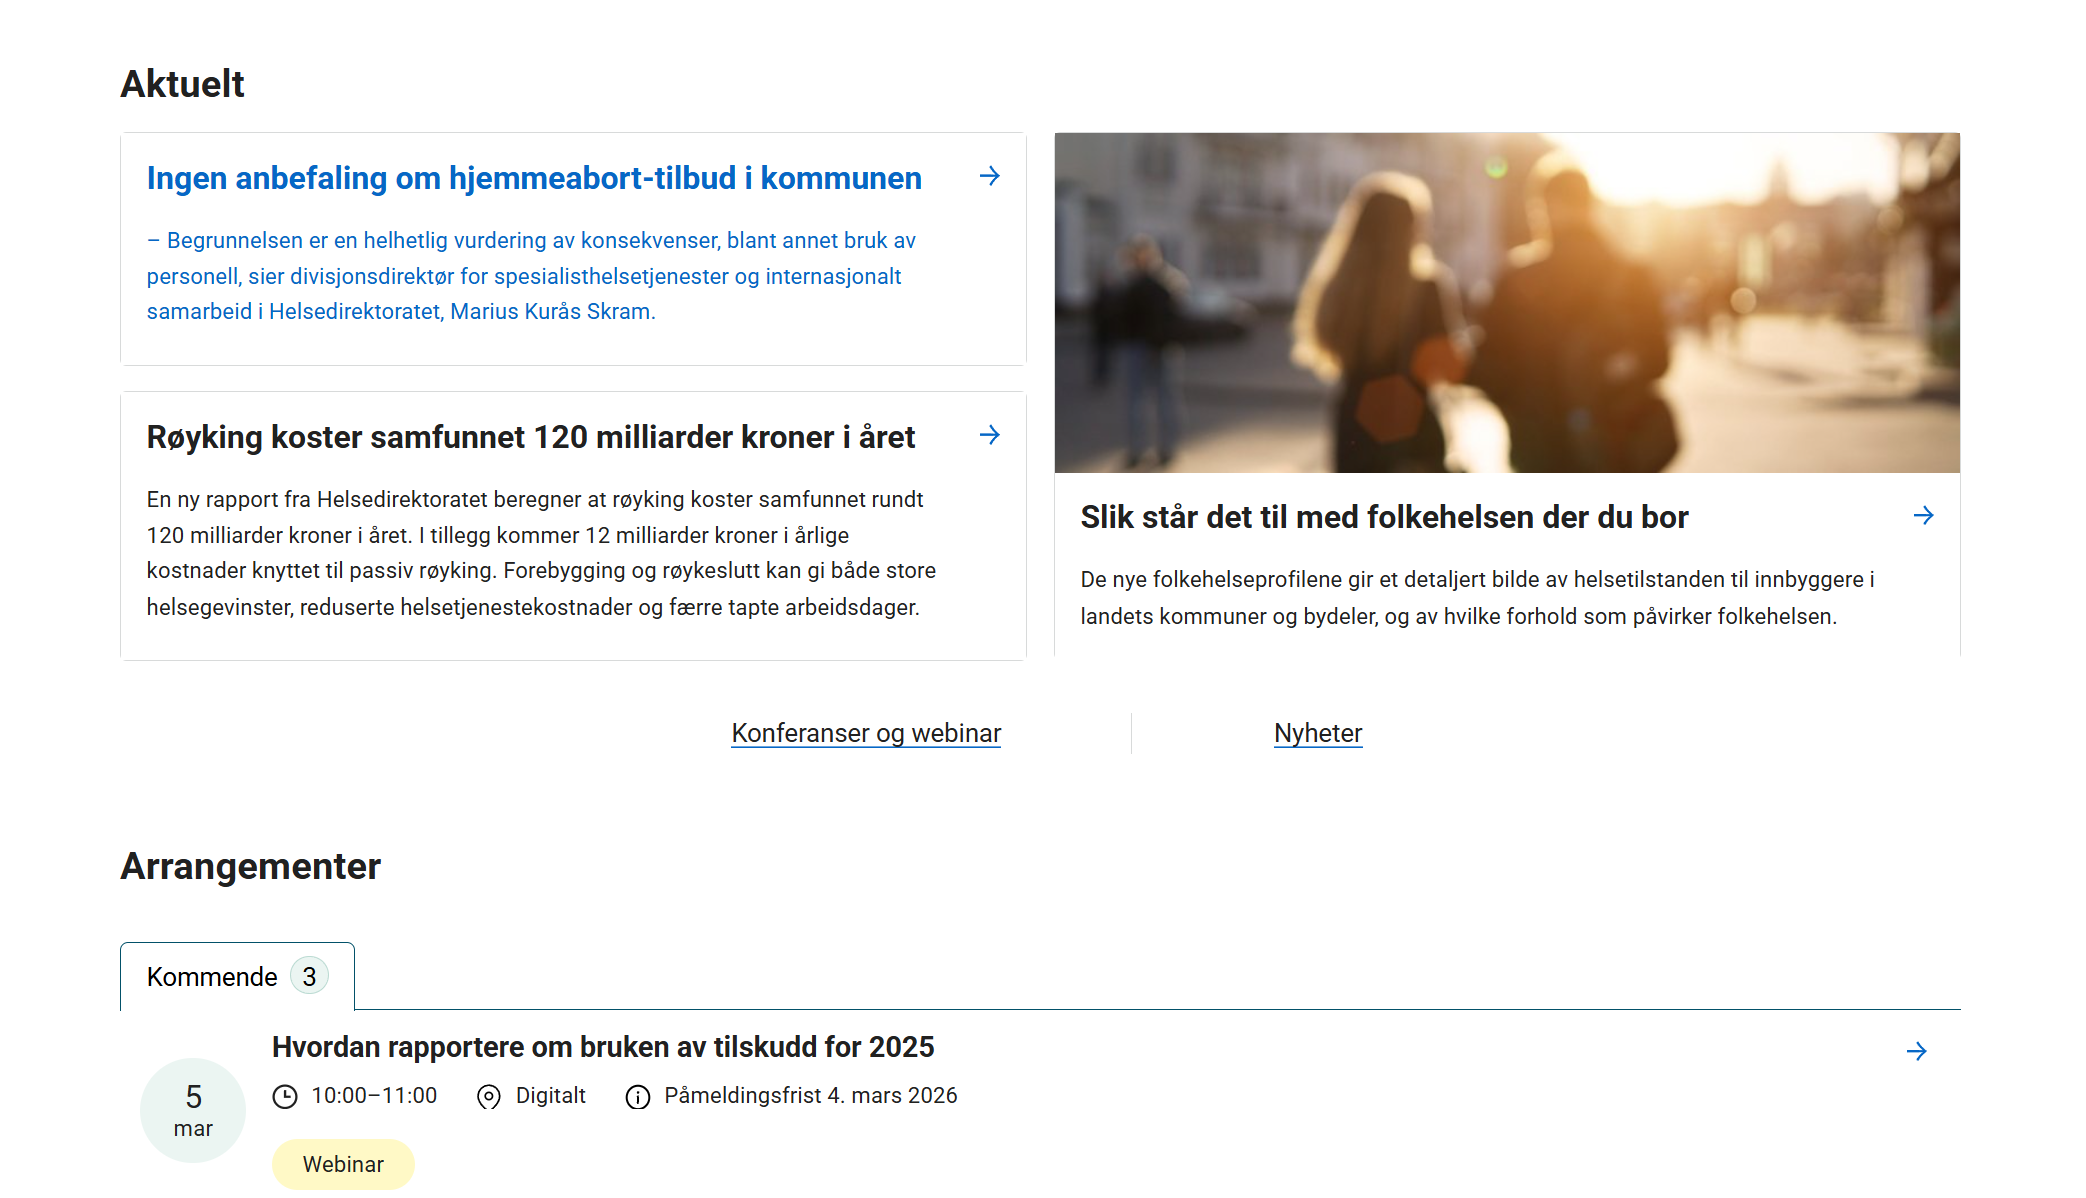
\includegraphics[width=\textwidth]{Images/helsedirektoratet.no/helsedir-forside-avgrensninger.png}
    \caption{Forsiden på helsedirektoratet.no som viser underinformasjon som vi ikke har tatt med i prototypen.}
    \label{fig:Helsedir-forside-avgrensninger}
\end{figure}



For å sikre gjennomførbarhet er arbeidet avgrenset til funksjonalitet som direkte påvirker søk og navigasjon. Innhold uten vesentlig relevans for informasjonsgjenfinning (f.eks.\ nyheter, arrangementer og annet redaksjonelt innhold) inngår ikke i prototypen som vist i figur \ref{fig:Helsedir-forside-avgrensninger}. Videre er prototypen avgrenset til et utvalg temasider som brukes som representative eksempler.

Ettersom prosjektet ikke har tilgang til en etablert brukerbase, gjennomføres evalueringen med et begrenset antall testbrukere. Resultatene må derfor tolkes som indikative for forbedringspotensial, ikke som endelig effekt i et produksjonsmiljø.

\subsection{Gruppens bakgrunn}

Prosjektet er organisert med tydelige roller, ansvarsområder og samarbeidsrutiner for å sikre strukturert og effektiv gjennomføring av arbeidet. Gruppen består av tre studenter fra 
Norwegian University of Technology and Science (NTNU) i Gjøvik\footnote{\url{https://www.ntnu.no/gjovik} besøkt 18. februar 2026.} med komplementær faglig kompetanse innen programvareutvikling, og arbeidet er organisert etter prinsipper fra smidig utviklingsmetodikk.


\subsubsection{Organisering}

En oversikt over prosjektgruppens organisering og rollefordeling er illustrert i \autoref{fig:organization-map}.

\begin{figure}[H]
    \centering
    \includesvg[width=0.7\textwidth]{Images/Figures/Group organization}
    \caption{Oversikt over prosjektgruppens struktur og rollefordeling.}
    \label{fig:organization-map}
\end{figure}


\subsubsection{Prosjektroller og ansvarsområder}

Prosjektgruppen er organisert etter etablerte roller inspirert av Scrum-rammeverket, med en tydelig fordeling av ansvar:

\subsubsection*{Roller:}

\begin{itemize}
    \item \textbf{Scrum master / prosjektleder: Fredrik Nymoen}
        \begin{itemize}
            \item Overordnet ansvar for fremdrift og koordinering av prosjektet.
            \item Kontaktpunkt mot produktansvarlig (product owner).
            \item Planlegging og gjennomføring av møter.
            \item Sikre rettferdig fordeling av arbeidsoppgaver i gruppen.
            \item Tilrettelegging for smidige arbeidsprosesser, inkludert sprintplanlegging og oppfølging.
        \end{itemize}
        
    \item \textbf{Utvikler: Amund Larsen}
        \begin{itemize}
            \item Ansvar for backend-utvikling.
            \item Ansvar for struktur, vedlikehold og kvalitetssikring av hovedrapporten i Overleaf, inkludert språklig og faglig konsistens.
            \item Bidrar til å sikre at prosjektets leveranser følger avtalte standarder og er i tråd med gruppekontrakten.
        \end{itemize}
        
    \item \textbf{Utvikler: Elling Bakås}
        \begin{itemize}
            \item Ansvar for frontend-utvikling.
            \item Ansvar for referatføring fra formelle møter, inkludert møter med produktansvarlig, veileder, sprintplanlegging og sprintgjennomganger.
        \end{itemize}

    \item \textbf{Product owner: Henrik Maurstad Jonasson}
        \begin{itemize}
            \item Representerer Helsedirektoratet som oppdragsgiver.
            \item Formidler oppdragsgivers behov, forventninger og visjon for prosjektet.
            \item Bidrar med innspill til prioritering av funksjonalitet og innhold i prosjektets produktbacklog.
        \end{itemize}
        
    \item \textbf{Veileder: Pål Anders Floor}
        \begin{itemize}
            \item Gir faglig og metodisk veiledning gjennom prosjektperioden.
            \item Bidrar med tilbakemeldinger på problemstilling, avgrensninger og rapportstruktur.
            \item Vurderer fremdrift og kvalitet på leveranser, og gir råd om videre prioriteringer.
            \item Diskuterer metodiske valg, evalueringsopplegg og akademisk presisjon.
            \item Fungerer som støtte ved utfordringer knyttet til gjennomførbarhet, risikohåndtering og planlegging.
        \end{itemize}
\end{itemize}

\subsubsection{Faglige ansvarsområder}

De faglige ansvarsområdene i prosjektet er fordelt i tråd med gruppemedlemmenes kompetanse og erfaring. Dette legger til rette for effektiv arbeidsdeling, samtidig som gruppen samarbeider tett på tvers av roller for å sikre helhetlige og konsistente løsninger.

\subsection{Rapportens oppbygning}
\label{sec:oppbygning}

Kapittel~\ref{sec:bakgrunn} presenterer bakgrunn og relevant teori knyttet til informasjonsgjenfinning, semantisk søk og navigasjon. Kapittel~\ref{sec:metode} beskriver forskningsdesign, datainnsamling, analyse og evalueringsopplegg, samt hvordan prosjektet er gjennomført i praksis. Deretter presenteres kartleggingen av dagens løsning (Del~I) i kapittel~\ref{sec:baseline}, før løsningen beskrives gjennom søkekomponenten (Del~II) i kapittel~\ref{sec:sok} og navigasjonsløsningen (Del~III) i kapittel~\ref{sec:navigasjon}. Resultater fra evalueringen presenteres i kapittel~\ref{sec:resultater} og diskuteres i kapittel~\ref{sec:diskusjon}. Avslutningsvis oppsummeres arbeidets bidrag og videre arbeid i kapittel~\ref{sec:konklusjon}.
